\documentclass{article}

\usepackage{geometry}
\usepackage{xeCJK}
\usepackage{amsmath}
\usepackage{tikz}
\usepackage{pgfplots}
\usepackage{pst-func}
% figure[H] float
\usepackage{float}
% subfigure
\usepackage{subcaption}
\usepackage{amssymb}
\usepackage{hyperref}
\usepackage{setspace}
% 字体底部样式:下划线、波浪线等
\usepackage{ulem}
% 修改公式编号
\usepackage{chngcntr}

% make cdot thicker,比 cdot 更粗的圆点
\makeatletter
\newcommand*\bigcdot{\mathpalette\bigcdot@{.5}}
\newcommand*\bigcdot@[2]{\mathbin{\vcenter{\hbox{\scalebox{#2}{$\m@th#1\bullet$}}}}}
\makeatother

% 设置行间距 1.5 倍
\renewcommand{\baselinestretch}{1.5}
% 自定义图片的标题:Figure -> 图
\renewcommand{\figurename}{图}
% 自定义表格的标题:Table -> 表
\renewcommand{\tablename}{表}

% 设置页大小和页边距,或者scale=0.8
\geometry{a4paper,left=3.18cm,right=3.18cm,top=2.54cm,bottom=2.54cm}
% 兼容
\pgfplotsset{compat=1.16}
% 中文默认没有斜体和粗体格式,开启伪斜体和指定黑体;
\setCJKmainfont[AutoFakeSlant, BoldFont=SimHei]{SimSun}
\usetikzlibrary{positioning}
% area of hatch,面积阴影部分
\usetikzlibrary{patterns}
% 箭头类型
\usetikzlibrary{arrows.meta}

\hypersetup{
    colorlinks,
    citecolor=black,
    filecolor=black,
    linkcolor=black,
    urlcolor=black
}
% 定义amsmath arccot, ch, sh
\DeclareMathOperator{\arccot}{arccot}
\DeclareMathOperator{\ch}{ch}
\DeclareMathOperator{\sh}{sh}
% 每个章节后,重置公式编号
\counterwithin*{equation}{section}

% 修改公式标签引用颜色
\def\eqref#1{{\color{blue}\hypersetup{linkcolor=blue} (\ref{#1}) }}
% 修改图片标签引用的颜色
\def\figureref#1{{\color{blue}\hypersetup{linkcolor=blue} (\ref{#1}) }}
% 修改跳转标签引用的颜色
\def\linkref[#1]#2{\hyperref[#1]{\color{blue}\ #2\ }}
% 引用 section 的章节号
\def\secref#1{\hyperref[#1]{\color{blue}[\ref{#1}节]}}

\begin{document}
  \tableofcontents
  \newpage

  \part{定积分的应用}
  \section{定积分的元素法}
    \paragraph{}
在前面的曲边梯形的面积问题里。将区间$[a,b]$分成长度为$\Delta x_i \; (i=1,2,\cdots,n)$的$n$个小区间。然后利用矩形的面积$f(x)dx$近似求得$\Delta A$的近似值,即
\begin{equation*}
  \Delta A \approx f(x)dx,
\end{equation*}
上式右端$f(x)dx$叫做\uwave{面积元素},记为$dA=f(x)dx$。于是
\begin{equation*}
  A \approx \sum f(x)dx
\end{equation*}
因此,
\begin{equation*}
  A = \lim\sum f(x)dx = \int_a^bf(x)dx.
\end{equation*}
这种方法通常叫做\uwave{元素法},或\uwave{微元法}。下面利用这个方法来讨论几何、物理中的一些问题。

  \section{定积分在几何学上的应用}
    \subsection{平面图形的面积}
\subsubsection{直角坐标情形}
\paragraph{}
应用定积分,可以计算一些比较复杂的平面图形的面积。

\paragraph{}
\textbf{例子1\;}计算抛物线$y^2=2x$与直线$y=x-4$所围成的图形的面积

\begin{figure}[H]
\centering
  % 直角坐标的定积分应用
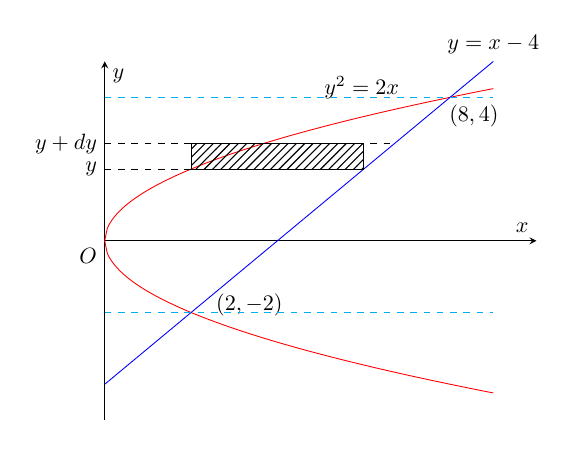
\begin{tikzpicture}[scale=0.8]
  \begin{axis}[clip=false,xmin=0, xmax=10,ymin=-5,ymax=5, grid=none,
    xtick=\empty, ytick=\empty, axis lines=middle,
    smooth, xlabel={$x$}, ylabel={$y$}]

    % 曲线: y^2=2x,y=x-4
    \addplot[draw=red,domain=0:9,samples=150] {sqrt(2*x)};
    \addplot[draw=red,domain=0:9,samples=150] {-sqrt(2*x)};
    \addplot[draw=blue,domain=0:9] {x-4};

    \node [right] at (2.4,-1.8) {$(2,-2)$};
    \node [below right] at (7.8,4) {$(8,4)$};

    \node [above] at (9,5) {$y=x-4$};
    \node [above left] at (7,3.74) {$y^2=2x$};

    \node [left] at (0,2.7) {$y + dy$};
    \node [left] at (0,2) {$y$};

    \draw [dashed] (0,2.7) -- (6.7,2.7);
    \draw [dashed] (0,2) -- (6,2);

    \draw [pattern=north east lines] (2,2) rectangle (6,2.7);


    \draw [dashed,draw=cyan] (0,-2) -- (9,-2);
    \draw [dashed,draw=cyan] (0,4) -- (9,4);

    % 原点
    \node [below left] at (0,0) {$O$};
  \end{axis}
\end{tikzpicture}

  \caption{抛物线与直线围成的面积}
\end{figure}

\paragraph{}
\textbf{解\;}为了确定图形的区间,先求出抛物线和直线的交点,解方程组
\begin{equation*}
  \left\{ \begin{array}{l}
    y^2 \;=\; 2x, \\
    y \;=\; x - 4,
  \end{array} \right.
\end{equation*}
得交点$(2,-2)$和$(8,4)$,从而知道这图形在直线$y=-2$及$y=4$之间。

\paragraph{}
现在,选取纵坐标$y$为积分变量,它的变化区间为$[-2,4]$(选取横坐标$x$为积分变量不方便)。

\paragraph{}
$[-2,4]$上任一小区间$[y,y+dy]$的窄条面积近似于高为$dy$、底为$\displaystyle(y+4)-\frac{1}{2}y^2$的窄矩形的面积,从而得到面积元素
\begin{equation*}
  dA = \big( y+4-\frac{1}{2}y^2 \big)dy.
\end{equation*}
以$\displaystyle\big( y+4-\frac{1}{2}y^2 \big)dy$为被积表达式,在闭区间$[-2,4]$上作定积分,便得所求的面积为
\begin{align*}
  A \;=&\; \int_{-2}^4\big( y+4-\frac{1}{2}y^2 \big)dy \\
  =&\; \big[ \frac{y^2}{2} + 4y - \frac{y^3}{6} \big]_{-2}^4 \\
  =&\; 18.
\end{align*}

\subsubsection{极坐标情形}
\paragraph{}

设由曲线$\rho=\varphi(\theta)$及射线$\theta=\alpha, \theta=\beta$围成一图形,现在要计算它的面积。这里,$\varphi(\theta)$在$[\alpha,\beta]$上连续,且$\varphi(\theta) \geq 0$。

\begin{figure}[H]
\centering
  % 极坐标的定积分应用
\begin{tikzpicture}[scale=1.5]
  \begin{polaraxis}[
    clip=false,ticks=none,grid=none,ylabel={$x$},
    axis lines=middle,x axis line style = {transparent},
    xmin=0,xmax=40,ymin=0,ymax=170,font=\tiny
  ]

    % ρ = φ(θ)
    \addplot[red,domain=10:40,samples=100] (x, {150+x/2)});
    \node [red,below right] at (40,175) {$\rho=\varphi(\theta)$};

    % alpha
    \addplot[blue,domain=0:155] (10, x);
    \addplot[blue,domain=0:10] (x,50);
    \node [blue] at (5,55) {$\alpha$};

    % beta
    \addplot[cyan,domain=0:170] (40, x);
    \addplot[cyan,domain=0:40] (x, 70);
    \node [cyan,rotate=15] at (15,75) {$\beta$};

    % θ
    \addplot[domain=0:20] (x, 90);
    \node [rotate=5] at (5,95) {$\theta$};

    % θ + dθ
    \addplot[domain=0:30] (x, 110);
    \node [right,rotate=5] at (5,107) {$\theta + d\theta$};

    \filldraw[pattern=north east lines] (0,0) -- (20,160) arc (20:30:32mm) -- cycle;

    % dθ
    \addplot[domain=20:30] (x, 130);
    \node [fill=white,right,rotate=25, inner sep = 1] at (25,130) {$d\theta$};

    % 原点
    \node [below left] at (0,0) {$O$};
  \end{polaraxis}
\end{tikzpicture}

  \caption{曲边扇形}
\end{figure}

\paragraph{}
由于当$\theta$在$[\alpha,\beta]$上变动时,极径$\rho=\varphi(\theta)$也随之变动,因此所求图形的面积不能直接利用扇形面积的公式$\displaystyle A=\frac{1}{2}R^2\theta$来计算。

\paragraph{}
取极角$\theta$为积分变量,它的变化区间为$[\alpha,\beta]$。相应于任一小区间$[\theta, \theta+d\theta]$的窄曲边扇形的面积可以用半径为$\rho=\varphi(\theta)$、中心角为$d\theta$的扇形的面积来近似代替,从而得到这窄曲边扇形面积的近似值,即曲边扇形的面积元素

\begin{equation*}
  dA = \frac{1}{2}[\varphi(\theta)]^2d\theta.
\end{equation*}

以$\displaystyle\frac{1}{2}[\varphi(\theta)]^2d\theta$为被积表达式,在闭区间$[\alpha,\beta]$上作定积分,便得所求曲边扇形的面积为
\begin{equation*}
  A = \int_\alpha^\beta\frac{1}{2}[\varphi(\theta)]^2d\theta.
\end{equation*}

\subsection{体积}
\subsubsection{旋转体的体积}
\paragraph{}
\uwave{旋转体}就是由一个平面图形绕这平面内一条直线,旋转一周而成的立体,这直线叫做\uwave{旋转轴}。

\begin{figure}[H]
\centering
  % 旋转体的体积, solid of revolution
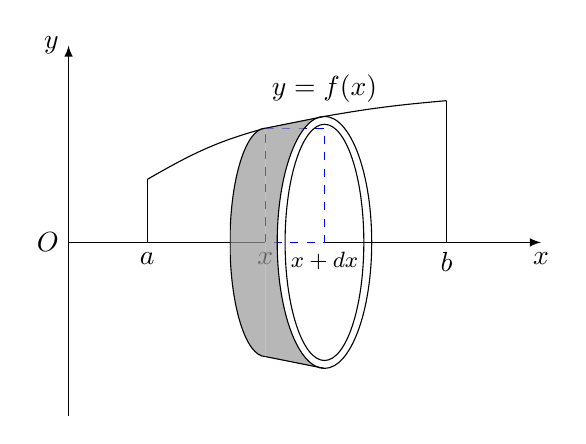
\begin{tikzpicture}[scale=1]
  % \draw [help lines] (-3,-3) grid (3,3);

  % 坐标
  \node[left] at (0,2.5) {$y$};
  \draw[-latex] (0,-2.2) -- (0,2.5);
  \node[below] at (6,0) {$x$};
  \draw (0,0) -- (2.5,0);
  \draw[-latex] (3.25,0) -- (6,0);
  \node[left] at (0,0) {$O$};

  % y=f(x)
  \node[above] at (3.25,1.65) {$y=f(x)$};
  \draw (1,0.8) to [out=30,in=195] (2.5,1.45);
  \draw (3.25,1.6) to [out=10,in=185] (4.8,1.8);

  % 端点
  \node[below] at (1,0) {$a$};
  \draw (1,0.8) -- (1,0);
  \node[below] at (4.8,0) {$b$};
  \draw (4.8,1.8) -- (4.8,0);

  \node[below] at (2.5,0) {$x$};
  \node[below] at (3.25,0) {\footnotesize $x + dx$};
  \draw[dashed, blue] (2.5,1.45) -- (3.25,1.45) -- (3.25,0) -- (2.5,0) -- (2.5,1.45);

  % ----------------------------------------------------------------------------

  % 左边椭圆和填充
  \begin{scope}
    \pgfsetfillopacity{0.7}
    \clip (2.05,-1.47) rectangle (2.501,1.47);
    \draw[fill=black!40] (2.5,0) ellipse [x radius=0.45cm,y radius=1.45cm];
  \end{scope}
  % 填充
  \begin{scope}
    \clip (2.4,-1.6) rectangle (3.24,1.6); % 3.25 --> 3.24,移除精度导致的黑线
    \pgfsetfillopacity{0.7}
    \path[fill=black!40,even odd rule] (2.5,1.45) -- (3.25,1.6) -- (3.25,-1.6) -- (2.5,-1.45) -- (2.5,1.45)
    (3.25,0) ellipse [x radius=0.6cm,y radius=1.6cm];
  \end{scope}

  % 右边椭圆
  \draw (3.25,0) ellipse [x radius=0.6cm,y radius=1.6cm];
  \draw (3.25,0) ellipse [x radius=0.5cm,y radius=1.5cm];

  % 椭圆上下边线
  \draw (2.5,1.45) -- (3.25,1.6);
  \draw (2.5,-1.45) -- (3.25,-1.6);
\end{tikzpicture}

  \caption{旋转体体积}
  \label{旋转体体积}
\end{figure}

\paragraph{}
上述旋转体都可以看作是由连续曲线$y=f(x)$、直线$x=a$、$x=b$及$x$轴所围成的曲边梯形绕$x$轴旋转一周而成的立体。现在下面用定积分来计算这种旋转体的体积。

\paragraph{}
取横坐标$x$为积分变量,它的变化区间为$[a,b]$。相应于$[a,b]$上的任一小区间$[x,x+dx]$的窄曲边梯形绕$x$轴旋转而成的薄片的体积近似于以$f(x)$为底半径、$dx$为高的扁圆柱体的体积(图 \figureref{旋转体体积}),即体积元素

\begin{equation}
  dV = \pi[f(x)]^2dx.
\end{equation}

\paragraph{}
以$\pi[f(x)]^2dx$为被积表达式,在闭区间$[a,b]$上作定积分,便得所求旋转体体积为

\begin{equation}
  V = \int_a^b\pi[f(x)]^2dx.
\end{equation}

\subsubsection{平行截面面积为已知的立体的体积}
\paragraph{}
从计算旋转体体积的过程中可以看出:如果一个立体不是旋转体,但却知道该立体上垂直于一定轴的各个截面的面积,那么,这个立体的体积也可以用定积分来计算。

\begin{figure}[H]
\centering
  % 已知平行截面面积的立体的体积
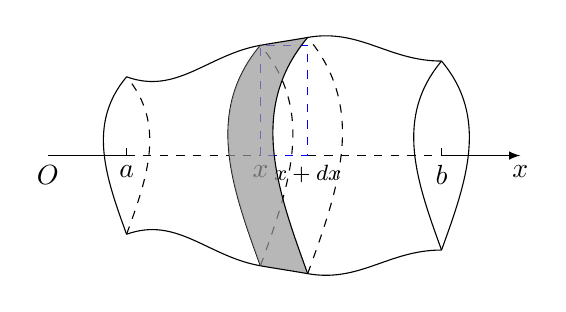
\begin{tikzpicture}[scale=1]
  % \draw [help lines] (0,-3) grid (6,3);

  \draw (0,0) -- (1,0);
  \draw[dashed] (1,0) -- (2.7,0);
  \draw[dashed] (3.3,0) -- (5,0);
  \draw[-latex] (5,0) -- (6,0);
  \node[below] at (0,0) {$O$};
  \node[below] at (1,0) {$a$};
  \draw (1,0) -- (1,0.1);
  \node[below] at (6,0) {$x$};
  \node[below] at (5,0) {$b$};
  \draw (5,0) -- (5,0.1);
  \node[below] at (2.7,0) {$x$};
  \node[below] at (3.3,0) {\footnotesize $x+dx$};
  \draw[dashed,blue] (2.7,0) -- (2.7,1.4) -- (3.3,1.4) -- (3.3,0) -- (2.7,0);

  % 左边
  \draw (1,-1) to [out=110,in=230] (1,1);
  \draw[dashed] (1,-1) to [out=70,in=-50] (1,1);

  % 左边的边框
  \draw (1,1) to [out=-20,in=190] (2.7,1.4);
  \draw (1,-1) to [out=20,in=170] (2.7,-1.4);

  % 中间 1
  \draw (2.7,-1.4) to [out=110,in=230] (2.7,1.4);
  \draw[dashed] (2.7,-1.4) to [out=70,in=-50] (2.7,1.4);

  % 阴影
  \begin{scope}
    \pgfsetfillopacity{0.7}
    \path[fill=black!40] (2.7,-1.4) to [out=110,in=230] (2.7,1.4) to [out=10,in=190] (3.3,1.5) to [out=230,in=110] (3.3,-1.5) to [out=170,in=-10] (2.7,-1.4);
  \end{scope}

  % 中间的边框
  \draw (2.7,1.4) to [out=10,in=190] (3.3,1.5);
  \draw (2.7,-1.4) to [out=-10,in=170] (3.3,-1.5);

  % 中间 2
  \draw (3.3,-1.5) to [out=110,in=230] (3.3,1.5);
  \draw[dashed] (3.3,-1.5) to [out=70,in=-50] (3.3,1.5);

  % 右边的边框
  \draw (3.3,1.5) to [out=10,in=180] (5,1.2);
  \draw (3.3,-1.5) to [out=-10,in=180] (5,-1.2);

  % 右边
  \draw (5,-1.2) to [out=110,in=230] (5,1.2);
  \draw (5,-1.2) to [out=70,in=-50] (5,1.2);
\end{tikzpicture}

  \caption{已知平行截面面积的立体的体积}
  \label{已知平行截面面积的立体的体积}
\end{figure}

\paragraph{}
如图\figureref{已知平行截面面积的立体的体积}所示,取上述定轴为$x$轴,并设该立体在过点$x=a$、$x=b$且垂直于$x$轴的两个平面之间。以$A(x)$表示过点$x$且垂直于$x$轴的截面面积。假定$A(x)$为$x$的已知的连续函数。这时,取$x$为积分变量,它的变化区间为$[a,b]$;立体中相应于$[a,b]$上任一小区间$[x,x+dx]$的一薄片的体积,近似于底面积为$A(x)$、高为$dx$的扁柱体的体积,即体积元素:
\begin{equation}
  dV = A(x)dx.
\end{equation}
以$A(x)dx$为被积表达式,在闭区间$[a,b]$上作定积分,便得所求立体的体积
\begin{equation}
  V = \int_a^bA(x)dx.
\end{equation}

\subsubsection{平面曲线的弧长}
\paragraph{}
圆的周长可以利用圆的内接正多边形的周长当边数无限增多时的极限来确定。现在用类似的方法来建立平面的连续曲线弧长的概念,从而应用定积分来计算弧长。

\begin{figure}[H]
\centering
  % 平面曲线的弧长
\begin{tikzpicture}[scale=0.8]
  \begin{axis}[clip=false,xmin=0, xmax=9,ymin=0,ymax=9, grid=none,
    xtick=\empty, ytick=\empty, axis lines=middle,
    smooth, xlabel={$x$}, ylabel={$y$}]

    % 曲线
    \addplot[domain=1.8:8] {-x^2/20 + x/6 + 1.5*ln(x - 1) + 4};

    \draw (1.8,3.8) -- (2.8,4.956) -- (3.8,5.46) -- (4.8,5.65) -- (5.8,5.64) -- (7.4,5.28) -- (8,5.05);
    \node[below] at (1.8,3.8) {$A=M_0$};
    \node[above left] at (2.8,4.956) {$M_1$};
    \node[above left] at (3.8,5.46) {$M_2$};

    \node[above] at (7.4,5.30) {$M_{n-1}$};
    \node[below] at (8,5.05) {$B=M_n$};

    % 原点
    \node [below left] at (0,0) {$O$};
  \end{axis}
\end{tikzpicture}

  \caption{平面曲线的弧长}
  \label{平面曲线的弧长}
\end{figure}

\paragraph{}
设$A, B$ 是曲线弧的两个端点。在弧$\overarc{AB}$上依次任取分点$A=M_0,M_1,M_2,\cdots,M_{i-1},M_i,\cdots$\\$,M_{n-1},M_n=B$,并依次连接相邻的分点得一折线(图\figureref{平面曲线的弧长})。当分点的数目无限增加且每个小段$\overarc{M_{i-1}M_i}$都缩向一点时,如果此折线的长$\displaystyle\sum_{i=1}^n|M_{i-1}M_i|$的极限存在,则称此极限为\uwave{曲线弧\text{$\overarc{AB}$}的弧长},并称此曲线弧$\overarc{AB}$是\uwave{可求长}的。

\paragraph{}
\textbf{定理\;}光滑曲线弧是可求长的。

\paragraph{}
下面利用定积分的元素法来讨论平面光滑曲线弧长的计算公式。

\paragraph{}
设曲线弧由参数方程

\begin{align}
\begin{split}
  \left\{\begin{array}{l} x=\varphi(t), \\ y = \psi(t) \end{array}\right. \; (\alpha \leq t \leq \beta)
\end{split}
\end{align}
给出,其中$\varphi(t), \psi(t)$在$[\alpha,\beta]$上具有连续导数,且$\varphi'(t), \psi'(t)$不同时为零。现在来计算这曲线弧的长度。

\paragraph{}
取参数$t$为积分变量,它的变化区间为$[\alpha,\beta]$。相应于$[\alpha,\beta]$上任一小区间$[t,t+dt]$的小弧段的长度$\Delta s$近似等于对应的弦的长度$\sqrt{(\Delta x)^2 + (\Delta y)^2}$。因为

\begin{align}
  \Delta x = \varphi(t+dt)-\varphi(t) \approx dx = \varphi'(t)dt, \\
  \Delta y = \psi(t+dt)-\psi(t) \approx dy = \psi'(t)dt,
\end{align}
所以,$\Delta s$的近似值(弧微分)即弧长元素为
\begin{align}
  ds \;=&\; \sqrt{(dx)^2 + (dy)^2} = \sqrt{\varphi'^2(t)(dt)^2 + \psi'^2(t)(dt)^2} \\
  \;=&\; \sqrt{\varphi'^2(t) + \psi'^2(t)}dt.
\end{align}
于是所求弧长为
\begin{equation}
  s = \int_\alpha^\beta\sqrt{\varphi'^2(t) + \psi'^2(t)}dt.
\end{equation}

\paragraph{}
当曲线弧由直角坐标方程
\begin{equation}
  y=f(x) \;\; (a \leq x \leq b)
\end{equation}
给出,其中$f(x)$在$[a,b]$上具有一阶连续导数,这时曲线弧有参数方程
\begin{align}
  \left\{\begin{array}{l}
    x = x, \\
    y = f(x)
  \end{array} \right. \; (a\leq x \leq b),
\end{align}
从而所求的弧长为

\begin{equation}
  s = \int_a^b\sqrt{1+y'^2}dx.
\end{equation}

\paragraph{}
当曲线弧由极坐标方程
\begin{equation}
  \rho = \rho(\theta) \;\; (\alpha \leq \theta \leq \beta)
\end{equation}
给出,其中$\rho(\theta)$在$[\alpha,\beta]$上具有连续导数,则由直角坐标与极坐标的关系可得
\begin{align}
  \left\{\begin{array}{ll}
    x \;= & \rho(\theta)\cos\theta, \\
    y \;= & \rho(\theta)\sin\theta
    \end{array}\right. \; (\alpha \leq \theta \leq \beta).
\end{align}
这就是以极角$\theta$为参数的曲线弧的参数方程。于是,弧长元素为
\begin{equation}
  ds = \sqrt{x'^2(\theta) + y'^2(\theta)}d\theta = \sqrt{\rho^2(\theta) + \rho'^2(\theta)}d\theta,
\end{equation}
从而所求弧长为
\begin{equation}
  s = \int_\alpha^\beta\sqrt{\rho^2(\theta) + \rho'^2(\theta)}d\theta.
\end{equation}

  \section{定积分在物理学上的应用}
    \subsection{变力沿直线所作的功}
\paragraph{}
如果物体在作直线运动的过程中有一个不变的力$F$作用在这个物体上,且这力的方向与物体运动的方向一致,那么在物体移动了距离$s$时,力$F$对物体所作的功为

\begin{equation}
  W = F \bigcdot s.
\end{equation}

\paragraph{}
如果物体在运动过程中所受到的力是变化的,这就会遇到变力对物体作功的问题。下面通过具体例子说明如何计算变力所作的功。

\begin{figure}[H]
\centering
  % 电荷做工
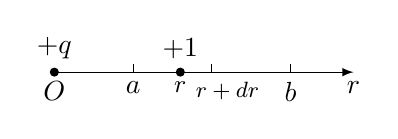
\begin{tikzpicture}[scale=1]
  \draw[-latex] (0,0) -- (3.8,0);
  \node[below] at (3.8,0) {$r$};

  \node[below] at (0,0) {$O$};
  \draw[fill=black] (0,0) circle (0.05cm);
  \node[above] at (0,0.05) {$+q$};

  \draw (1,0) -- (1,0.1);
  \node[below] at (1,0) {$a$};

  \node[below] at (1.6,0) {\small $r$};
  \node[above] at (1.6,0.05) {$+1$};
  \draw[fill=black] (1.6,0) circle (0.05cm);

  \draw (2,0) -- (2,0.1);
  \node[below] at (2.2,0) {\footnotesize $r+dr$};

  \draw (3,0) -- (3,0.1);
  \node[below] at (3,0) {$b$};
\end{tikzpicture}

  \caption{电荷做功}
  \label{电荷做功}
\end{figure}

\paragraph{}
\textbf{例1\;}把一个带电荷量$+q$的点电荷放在$r$轴上坐标原点$O$处,它产生一个电场。这个电场对周围的电荷有作用力。由物理学知道,如果有一个单位正电荷放在这个电场中距离原点$O$为$r$的地方,那么电场对它的作用力的大小为
\begin{equation}
  F = k\frac{q}{r^2} \; (k\text{是常数}).
\end{equation}

见图\figureref{电荷做功},当这个单位正电荷在电场中从$r=a$处沿$r$轴移动到$r=b \, (a<b)$处时,计算电场力$F$对它所作的功。

\paragraph{}
\textbf{解\;}在上述移动过程中,电场对这单位正电荷的作用力是变的,取$r$为积分变量,它的变化区间为$[a,b]$。设$[r,r+dr]$为$[a,b]$上的任一小区间。当单位正电荷从$r$移动到$r+dr$时,电场力对它所作的功近似于$\displaystyle\frac{kq}{r^2}dr$,即功元素为
\begin{equation}
  dW = \frac{kq}{r^2}dr.
\end{equation}

\paragraph{}
于是所求的功为
\begin{equation}
  W = \int_a^b\frac{kq}{r^2}dr = kq\big[ -\frac{1}{r} \big]_a^b = kq\big( \frac{1}{a} - \frac{1}{b} \big).
\end{equation}

\paragraph{}
在计算静电场中某点的电位时,要考虑将单位正电荷从该点处($r=a$)移到无穷远处时,电场力所作的功$W$。此时,电场力对单位正电荷所作的功就是反常积分:

\begin{equation}
  W = \int_a^{+\infty}\frac{kq}{r^2}dr = \big[ -\frac{kq}{r} \big]_a^{+\infty} = \frac{kq}{a}.
\end{equation}

\subsection{水压力}
\paragraph{}
在水深为$h$处的压强为$p = \rho gh$,这里$\rho$是水的密度,$g$是重力加速度。如果有一面积为$A$的平板水平地放置在水深为$h$处,那么,平板一侧所受的水压力为

\begin{equation}
  P = p \bigcdot A.
\end{equation}

\paragraph{}
如果平板铅直放置在水中,那么,由于水深不同的点处压强$p$不相等,平板一侧所受的水压力就不能用上述方法计算。下面举例说明它的计算方法。

\paragraph{}
\textbf{例2\;}一个横着放着的圆柱形水桶,桶内盛有半桶水(图\linkref[横放着的圆柱水桶水压a]{(\ref{横放着的圆柱水桶水压} - a)})。设桶的底半径为$R$,水的密度为$\rho$,计算桶的一个端面上所受的压力。

\begin{figure}[h]
\centering
  %------- 第1行 -------
  \begin{subfigure}[t]{0.42\linewidth}
    \centering
      % 水压力例子(a)
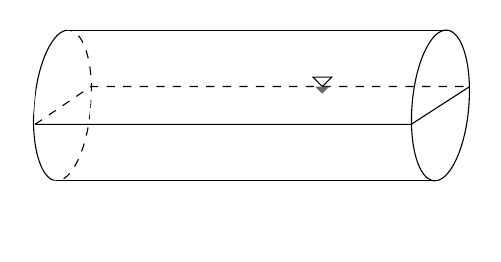
\begin{tikzpicture}[scale=0.6]
  % \draw [help lines] (-1,-3) grid (9,3);

  % 左椭圆
  \begin{scope}
    \clip[rotate=-5] (-0.6,-1.6) rectangle (0,1.6);
    \draw[rotate=-5] (0,0) ellipse [x radius=0.6cm,y radius=1.6cm];
  \end{scope}
  \begin{scope}
    \clip[rotate=-5] (0,-1.6) rectangle (0.6,1.6);
    \draw[dashed,rotate=-5] (0,0) ellipse [x radius=0.6cm,y radius=1.6cm];
  \end{scope}

  % 上下边框
  \draw (0.139,1.593) -- (8.139,1.593);
  \draw (-0.139,-1.593) -- (7.861,-1.593);

  % 水面
  \draw (-0.58,-0.4) -- (7.38,-0.4) -- (8.62,0.4);
  \draw[dashed] (-0.58,-0.4) -- (0.6,0.4) -- (8.62,0.4);

  \draw (5.5,0.4) -- (5.3,0.6) -- (5.7,0.6) -- (5.5,0.4);
  \path[fill=black!60] (5.5,0.25) -- (5.35,0.4) -- (5.65,0.4) -- (5.5,0.25);

  % 右椭圆
  \draw[rotate around={-5:(8,0)}] (8,0) ellipse [x radius=0.6cm,y radius=1.6cm];

  % 空白,提升高度,底部的 padding
  \draw[white] (0,-2.7) -- (0.01,-2.7);
\end{tikzpicture}

      \caption{}
      \label{横放着的圆柱水桶水压a}
  \end{subfigure}
  \begin{subfigure}[t]{0.42\linewidth}
    \centering
      % 水压力例子(b)
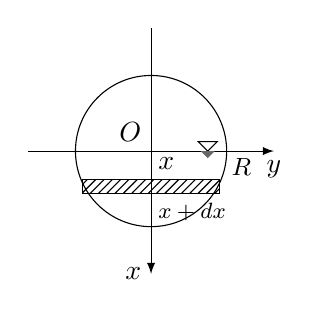
\begin{tikzpicture}[scale=0.6]
  \node[below] at (2.6,0) {$y$};
  \draw[-latex] (-2.6,0) -- (2.6,0);
  \node[left] at (0,-2.6) {$x$};
  \draw[-latex] (0,2.6) -- (0,-2.6);
  \draw (0,0) circle (1.6cm);

  \draw (1.2,0) -- (1,0.2) -- (1.4,0.2) -- (1.2,0);
  \path[fill=black!60] (1.2,-0.15) -- (1.05,0) -- (1.35,0) -- (1.2,-0.15);

  \node[above left] at (0,0) {$O$};
  \node[below right] at (1.5,0.05) {\small $R$};

  \node[above right] at (-0.05,-0.6) {$x$};

  \draw[pattern=north east lines] (-1.45,-0.6) -- (1.45,-0.6) -- (1.45,-0.9) -- (-1.45,-0.9) -- (-1.45,-0.6);
  \node[below right] at (-0.05,-0.9) {\footnotesize $x+dx$};
\end{tikzpicture}

      \caption{}
      \label{横放着的圆柱水桶水压b}
  \end{subfigure}

  \caption{横放着的圆柱水桶水压}
  \label{横放着的圆柱水桶水压}
\end{figure}

\paragraph{}
\textbf{解\;}桶的一个端面是圆片,所以现在要计算的是当水平面通过圆心时,铅直放置的一个半圆片的一侧所受到的水压力。

\paragraph{}
如图\linkref[横放着的圆柱水桶水压b]{(\ref{横放着的圆柱水桶水压} - b)},在这个圆片上取过圆心且铅直向下的直线为$x$轴,过圆心的水平线为$y$轴。对这个坐标系来讲,所讨论的半圆的方程为$x^2+y^2=R^2 \; (0\leq x\leq R)$。取$x$为积分变量,它的变化区间为$[0,R]$。设$[x,x+dx]$为$[0,R]$上的任一小区间,半圆片上相应于$[x,x+dx]$的窄条上各点处的压强近似于$\rho gx$,这窄条的面积近似于$\displaystyle 2\sqrt{R^2-x^2}dx$。因此,这窄条一侧所受水压力的近似值,即压力元素为

\begin{equation}
dP = 2\rho gx \sqrt{R^2-x^2}dx.
\end{equation}

于是所求压力为
\begin{align}
  P \;=&\; \int_0^R 2\rho gx \sqrt{R^2-x^2}dx = -\rho g\int_0^R(R^2-x^2)^{1/2}d(R^2-x^2) \\
  \;=&\; -\rho g\big[ \frac{2}{3}(R^2-x^2)^{3/2} \big]_0^R = \frac{2\rho g}{3}R^3.
\end{align}

\subsection{引力}
\paragraph{}
质量分别为$m_1, m_2$,相距为$r$的两质点间的引力的大小为
\begin{equation}
  F = G\frac{m_1m_2}{r^2},
\end{equation}
其中$G$为引力系数,引力的方向沿着两质点的连线方向。

\paragraph{}
如要计算一根细棒对一个质点的引力,那么由于细棒上各点与该质点的距离是变化的,且各点对该质点的引力的方向也是变化的,因此就不能用上述公式来计算。下面举例说明它的计算方法。

\paragraph{}
\textbf{例3\;}设有一长度为$l$、线密度为$\mu$的均匀细直棒,在其中垂线上距棒$a$单位处有一质量为$m$的质点$M$。试计算该棒对质点$M$的引力。

\begin{figure}[H]
\centering
  % 引力应用
\begin{tikzpicture}[scale=0.6]

  \node[left] at (0,5) {$y$};
  \draw[-latex] (0,-5) -- (0,5);
  \node[below] at (7,0) {$x$};
  \draw[-latex] (0,0) -- (7,0);

  % M
  \node[below right] at (4,0) {$M$};
  \draw[fill=black] (4,0) circle (0.08cm);
  \draw[-latex] (4,0) -- (0,2);

  % y
  \node[left] at (-0.15,2) {$y$};
  \draw (0,2) -- (-0.15,2);

  \node[left] at (-0.15,2.6) {$y+dy$};
  \draw (0,2.6) -- (-0.15,2.6);

  \node[below] at (2,0) {$a$};

  \draw[line width=0.05cm] (0,3.5) -- (0,-3.5);
  \node[left] at (0,3.5) {$\frac{l}{2}$};
  \node[left] at (0,-3.5) {$-\frac{l}{2}$};

  \node[above right] at (2,1) {$r$};

  % 原点
  \node [left] at (0,0) {$O$};
\end{tikzpicture}

  \caption{引力}
  \label{引力}
\end{figure}

\textbf{解\;}取坐标系如图\figureref{引力}所示,使棒位于$y$轴上,质点$M$位于$x$轴上,棒的中点为原点$O$。取$y$为积分变量,它的变化区间为$\big[-\frac{l}{2}, \frac{l}{2} \big]$。设$[y, y+dy]$为$\big[-\frac{l}{2}, \frac{l}{2} \big]$上任一小区间,把细直棒上相应于$[y,y+dy]$的一小段近似地看成质点,其质量为$\mu dy$,与$M$相距$\displaystyle r=\sqrt{a^2+y^2}$。因此可以按照两质点间的引力计算公式求出这小段细直棒对质点$M$的引力$\Delta F$的大小为

\begin{equation}
  \Delta F \approx G\frac{m\mu dy}{a^2+y^2},
\end{equation}

\paragraph{}
从而求出$\Delta F$在水平方向分力$\Delta F_x$的近似值,即细直棒对质点$M$的引力在水平方向分力$F_x$的元素为

\begin{equation}
  dF_x = -G\frac{am\mu dy}{(a^2+y^2)^{\frac{3}{2}}},
\end{equation}

于是得引力在水平方向分力为
\begin{align}
  F_x \;=&\; - \int_{-\frac{l}{2}}^{\frac{l}{2}} \frac{Gam\mu}{(a^2+y^2)^{\frac{3}{2}}} dy \\
  \;=&\; -\frac{2Gm\mu l}{a} \bigcdot \frac{1}{\sqrt{4a^2+l^2}}.
\end{align}
由对称性知,引力在铅直方向分力为$F_y=0$.

\paragraph{}
当细直棒的长度$l$很大时,可视$l$趋于无穷。此时,引力的大小为$\displaystyle \frac{2Gm\mu}{a}$,方向与细棒垂直且由$M$指向细棒。

\end{document}
